\section{The NASA almond}
\label{sec:almond}

Our last shape is the NASA almond \cite{woo1993}, a standard test case in computational electromagnetics. It is a smooth body of length $L = 0.2524$\,m with a rounded rear and a sharp tip, whose cross-sections are ellipses with axis ratio $3{:}1$. We place the almond with its long axis along $x$, the tip at positive $x$ and its mid-plane in $z = 0$. It is symmetric under the mirrors $y\to-y$ and $z\to-z$. The almond combines the two difficulties met so far: a singular set close to the surface, as for a thin torus, and a point where it reaches the surface, as at the edges of the cube.

\subsection{Sources on the mid-plane}

By \autoref{sec:focal} the sources lie on the mid-plane and cluster towards the focal curve, which runs at the fraction $\eta_F = 0.943$ of the half-width (\autoref{fig:almondlayout}). They are point dipoles arranged in rows. In the front half a row follows the outline of the mid-plane section at a fixed fraction $\eta$ of the half-width, and in the rear half it continues as the ellipse through the same point of the widest section that is confocal with the focal ellipse. We use $n_{\mathrm{mid}}$ rows in the middle of the section and $n_F+1$ rows at
\begin{equation}
  \eta_j = \eta_F - 2\,(1-\eta_F)\,2^{-j}, \qquad j = 0,\dots,n_F,
\end{equation}
which approach the focal curve geometrically from the inside, and we write $n_{\mathrm{mid}}{:}n_F$ for a layout. The rows in the middle lie at the fractions $\bigl(\eta_F - 3(1-\eta_F)\bigr)\cos\bigl((i+\tfrac12)\pi/(2n_{\mathrm{mid}})\bigr)$, $i = 0,\dots,n_{\mathrm{mid}}-1$. Along a row the spacing of the sources is a fixed multiple of the local distance to the surface, and the boundary points follow the same rule with half that multiple or less, such that there are at least $2.5$ equations for each unknown. Sources and boundary points thus refine together towards the rim.

As for the cube, we use the symmetry. An incident wave is split into its four parts of definite parity under the two mirrors, and each part is solved on one quarter of the body. A source on the mid-plane then keeps three of its six dipole components: the two electric components in the plane and the magnetic component normal to it for the classes that are even under $z\to-z$, and the other three for the odd classes.

\begin{figure}[htbp]
  \centering
  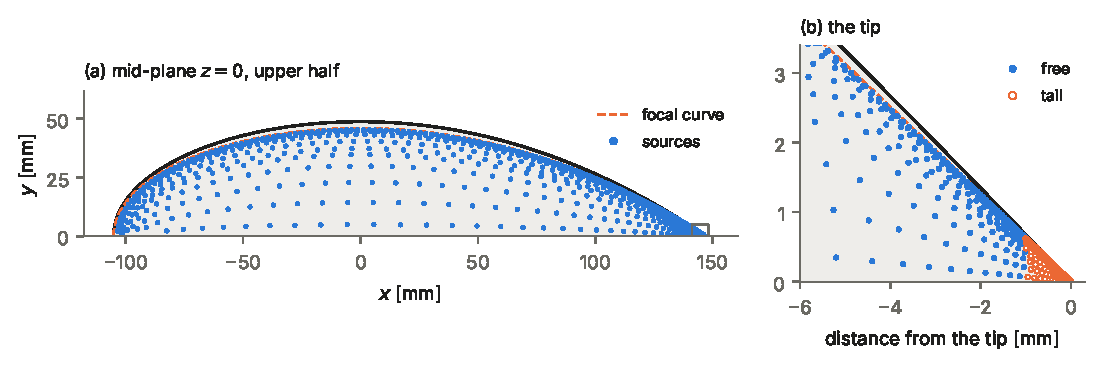
\includegraphics[width=0.8\textwidth]{fig_almond_layout.pdf}
  \caption{Source layout of the almond in the mid-plane $z = 0$ (one half shown). The rows of point dipoles cluster towards the focal curve (dashed), which runs within $6\%$ of the rim, and continue into the tip as a tail.}
  \label{fig:almondlayout}
\end{figure}

\subsection{A tail at the tip}

The focal curve reaches the surface at the tip, which is the vertex of an elliptic cone with half-angles $34.09^\circ$ and $12.71^\circ$. The field of a conducting cone behaves like $r^{\nu-1}$ at distance $r$ from the vertex \cite{desmedt1986}. For this cone we computed the smallest exponent $\nu = 0.2996$ (\ref{app:cone}), so the electric field grows like $r^{-0.70}$ towards the tip.

The free source rows stop $1$\,mm from the tip. The singular term belongs to the parity class that is even under both mirrors, and for this class the cut-off leaves a boundary residual of $19\%$, with a cross-section at oblique angles that is wrong by up to $1.2$\,dB. Adding sources does not help. The remedy is the tail of \autoref{sec:tail}. Each row is continued to within $10^{-4}$\,mm of the tip, and the continued dipoles of a row are tied together with the weights $(r/r_{\mathrm{cut}})^{\nu+2}$ for electric and $(r/r_{\mathrm{cut}})^{\tau+2}$ for magnetic dipoles, where $r_{\mathrm{cut}}$ is the distance of the cut-off from the tip. We use the two smallest electric exponents $\nu$ and the smallest magnetic exponent $\tau$ of the parity class, each with its own coefficient for every row and dipole component, which adds $50$ unknowns per class. For the class that is even under both mirrors these are $\nu = 0.2996$ and $1.464$ and $\tau = 1.975$ (\autoref{tab:coneexp}). With the tail the residual of this class falls from $19\%$ to $0.034\%$.

\subsection{Results}

We first consider the wave that travels along $-x$ and meets the tip first (nose-on incidence), polarised along $y$, at $1.19$\,GHz, where the almond is one wavelength long. Here the sources are spaced along the rows at $0.7$ times their distance to the surface. Measured against the finest layout, $8{:}5$ with $4791$ unknowns, the layouts $5{:}2$ and $6{:}3$, with $2103$ and $2937$ unknowns, differ by $2.8\times10^{-4}$ and $5.6\times10^{-5}$. Refining the reference layout in three different ways changes its field by less than $10^{-5}$.

The quantity of practical interest is the monostatic radar cross-section as a function of the azimuth in the plane of the almond, for the polarisations HH (electric field in the plane) and VV (electric field along $z$). The factorisation of a parity class serves all look angles, so one frequency, with $361$ look angles from $0^\circ$ to $180^\circ$ and both polarisations, takes about two minutes with the layout $6{:}3$. We compare with the Austin RCS Benchmark Suite \cite{kelley2020}, which provides measurements of this almond and a reference simulation with $397{,}674$ unknowns at $3.5$, $5.125$, $7$ and $10.25$\,GHz. At the highest frequency the almond is $8.6$ wavelengths long. We use the same layout $6{:}3$ at all four frequencies, with a closer spacing of the sources along the rows ($0.5$ times the distance to the surface instead of $0.7$), which gives $4193$ unknowns for each of the four parity classes.

\autoref{fig:almondbench} shows the three sets of curves, and \autoref{tab:almondbench} lists the mean absolute difference in decibels over the look angles. The MFS differs from the reference simulation by $0.04$ to $0.14$\,dB for HH and by $0.01$ to $0.02$\,dB for VV. For comparison, the two finest meshes of the reference simulation differ from each other by $0.07$ and $0.02$\,dB at $7$\,GHz \cite{kelley2020}. Both simulations differ from the measurements by $0.6$ to $1.8$\,dB, which is the level at which the measurements are stated to agree with simulation, $\pm1$\,dB for HH and $\pm2$\,dB for VV \cite{kelley2020}.

\begin{table}[htbp]
  \centering
  \caption{NASA almond, monostatic cross-section: mean absolute difference in dB between the MFS (layout $6{:}3$) and the reference simulation of the Austin benchmark \cite{kelley2020}, over $361$ look angles.}
  \label{tab:almondbench}
  \begin{tabular}{lrrrr}
    \toprule
    Frequency [GHz] & 3.5 & 5.125 & 7 & 10.25 \\
    \midrule
    HH & 0.043 & 0.055 & 0.072 & 0.140 \\
    VV & 0.011 & 0.013 & 0.016 & 0.024 \\
    \bottomrule
  \end{tabular}
\end{table}

\begin{figure}[htbp]
  \centering
  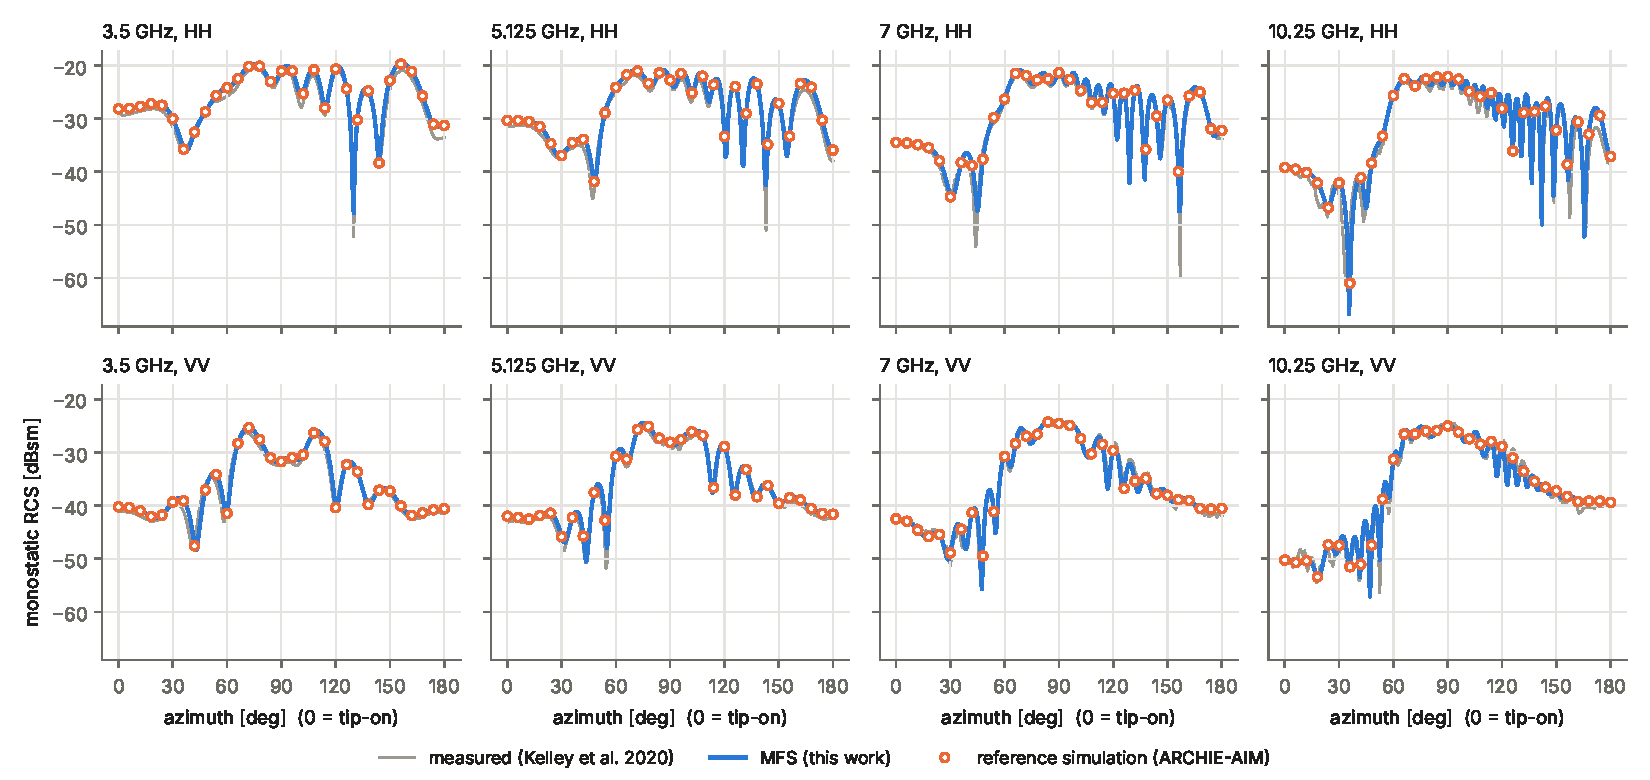
\includegraphics[width=0.9\textwidth]{fig_almond_benchmark.pdf}
  \caption{NASA almond: monostatic radar cross-section against azimuth ($0^\circ$ is nose-on) at four frequencies, HH and VV. MFS, reference simulation and measurements of the Austin benchmark \cite{kelley2020}.}
  \label{fig:almondbench}
\end{figure}

The largest pointwise differences from the reference simulation occur in deep nulls of the HH cross-section, where the reference itself is least certain: its two finest meshes differ by up to $0.5$\,dB near the nulls \cite{kelley2020}. The largest difference is $4.3$\,dB at $10.25$\,GHz and $35.5^\circ$, in a null at $-66.7$\,dBsm. The MFS is converged there, since the layouts $6{:}3$ and $8{:}5$ differ by $0.024$\,dB in this null. The difference is one of position and not of depth: shifting the MFS curve by $0.1^\circ$ halves its distance from the reference samples around this sharp null.

In summary, the MFS agrees with the reference simulation to $0.14$\,dB or better on average. At $7$\,GHz, where the comparison can be made, this is the size of the difference between the two finest meshes of that simulation. The MFS needs four systems of about $4200$ unknowns each where the reference uses $397{,}674$ unknowns. The computing time at the lowest frequency is compared with the boundary element method in the next section.
